Current machine learning algorithms' performance depend heavily on the particular features of the data chosen as inputs. For example, document classification (such as marking emails as spam or not) can be performed by breaking down the input document into bag-of-words or n-grams as features. Choosing the correct feature representation of input data, or feature engineering, is a way that people can bring prior knowledge of a domain to increase an algorithm's computational performance and accuracy. To move towards general artificial intelligence, algorithms need to be less dependent on this feature engineering and better learn to identify the explanatory factors of input data on their own \cite{bengio12}.

\section{Representation Learning}
Deep learning approaches (also known as deep architectures) move in this direction by capturing a good representation of input data by using compositions of non-linear transformations. A good representation can be defined as one that disentangles underlying factors of variation for input data \cite{bengio13}. Deep learning approaches can find useful abstract representations of data across many domains: it has had great commercial success powering most of Google and Microsoft's current speech recognition, image classification, natural language processing, object recognition, etc. Facebook is also planning on using deep learning approaches to understand its users\footnote{http://www.technologyreview.com/news/519411/facebook-launches-advanced-ai-effort-to-find-meaning-in-your-posts/}. Deep learning has been so impactful in industry that MIT Technology Review named it as a top-10 breakthrough technology of 2013\footnote{http://www.technologyreview.com/featuredstory/513696/deep-learning/}.

The central idea to building a deep architecture is to learn a hierarchy of features one level at a time where the input to one computational level is the output of the previous level for an arbitrary number of levels. Otherwise, shallow representations (such as regression or support vector machines) go directly from input data to output classification.

One good analogue for deep architectures is neurons in the brain (a motivation for artificial neural networks) - the output of a group of neurons is agglomerated as the input to more neurons to form a hierarchical layer structure. Each layer \(N\) is composed of \(h\) computational nodes that connect to each computational node in layer \(N+1\).

\begin{figure}[h!]
  \centering
    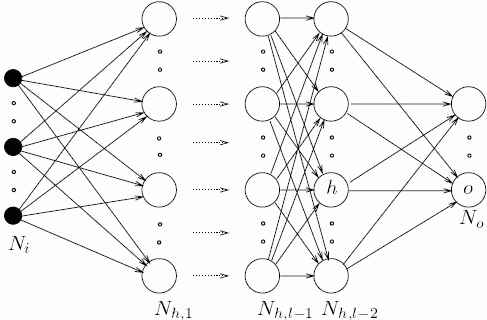
\includegraphics[width=0.7\textwidth]{neural_net}
\caption{An example deep architecture.}
\end{figure}

\section{Interpretations of Deep Architectures}
There are two main ways to interpret the computation performed by these layered deep architectures:

\begin{itemize}
\item \emph{Probabilistic graphical models} have nodes in each layer that are considered as latent random variables. In this case, you care about the probability distribution of the input data \(x\) and the hidden latent random variables \(h\) that describe the input data in the joint distribution \(p(x,h)\). These latent random variables describe a distribution over the observed data.
\item \emph{Direct encoding models} have nodes in each layer that are considered as computational units. This means each node \(h\) performs some computation (normally nonlinear like a sigmoidal function, hyperbolic tangent nonlinearity, or rectifier linear unit) given its inputs from the previous layer.
\end{itemize}

To get started, principal component analysis (PCA) is a simple feature extraction algorithm that can span both of these interpretations. PCA learns a linear transform \(h = f(x) = W^T x + b\) where \(W\) is a weight matrix for the inputs \(x\) and \(b\) is a bias term. The columns of the \(dx \times dh\) matrix \(W\) form an orthogonal basis for the \(dh\) orthogonal directions of greatest variance in the input training data \(x\). The result is \(dh\) features that make representation layer \(h\) that are decorrelated. 

\begin{figure}[h!]
  \centering
    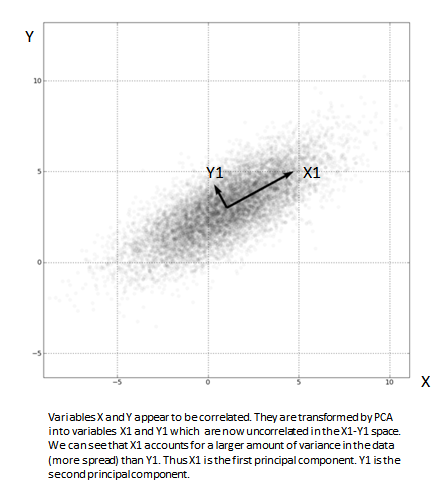
\includegraphics[width=0.65\textwidth]{pca}
\caption{Principal component analysis.}
\end{figure}

From a probabilistic viewpoint, PCA is simply finding the principal eigenvectors of the covariance matrix of the data. This means that you are finding which features of the input data can explain away the most variance in the data\cite{bach05}. From an encoding viewpoint, PCA is performing a linear computation over the input data to form a hidden representation h that has a lower dimensionality than the data.

Note that because PCA is a linear transformation of the input \(x\), it cannot really be stacked in layers because the composition of linear operations is just another linear operation. There would be no abstraction benefit of multiple layers. To show these two methods of analysis, this section will examine stacking Restricted Boltzmann Machines (RBM) from a probability viewpoint and nonlinear auto-encoders from a direct encoding viewpoint.

\subsection{Probabilistic models: restricted boltzmann machine (RBM)}
A Boltzmann machine is a network of symmetrically-coupled binary random variables or units. This means that it is a fully-connected, undirected graph. This graph can be divided into two parts:

\begin{enumerate}
\item The visible binary units \(x\) that make up the input data and
\item The hidden or latent binary units \(h\) that explain away the dependencies between the visible units \(x\) through their mutual interactions.
\end{enumerate}

\begin{figure}[h!]
  \centering
    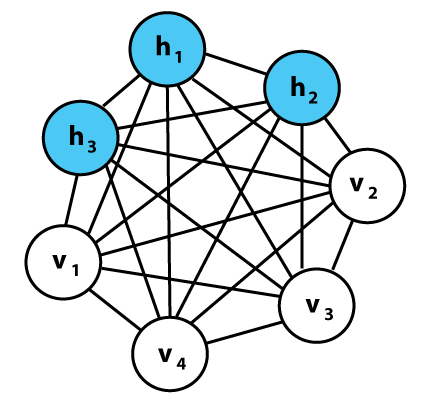
\includegraphics[width=0.45\textwidth]{boltzmann_machine}
\caption{A graphical representation of a Boltzmann machine. Each undirected edge represents dependency; in this example there are 3 hidden units and 4 visible units.}
\end{figure}

Boltzmann machines describe this pattern of interaction through the distribution over the joint space \([x,h]\) with the energy function: 
\[\varepsilon_\Theta^{BM} (x,h) = -\frac{1}{2} x^T Ux - \frac{1}{2} h^T Vh - x^T Wh - b^T x - d^T h\]
Where the model parameters \(\Theta\) are \(\left\{U,V,W,b,d\right\}\).

Trying to evaluate conditional probabilities over this fully connected graph ends up being an intractable problem. For example, computing the conditional probability of hidden variable given the visibles, \(P(h_i | x)\), requires marginalizing over all the other hidden variables. This would be evaluating a sum with \(2dh - 1\) terms.

However, we can restrict the graph from being fully connected to only containing the interactions between the visible units \(x\) and hidden units \(h\). 

\begin{figure}[h!]
  \centering
    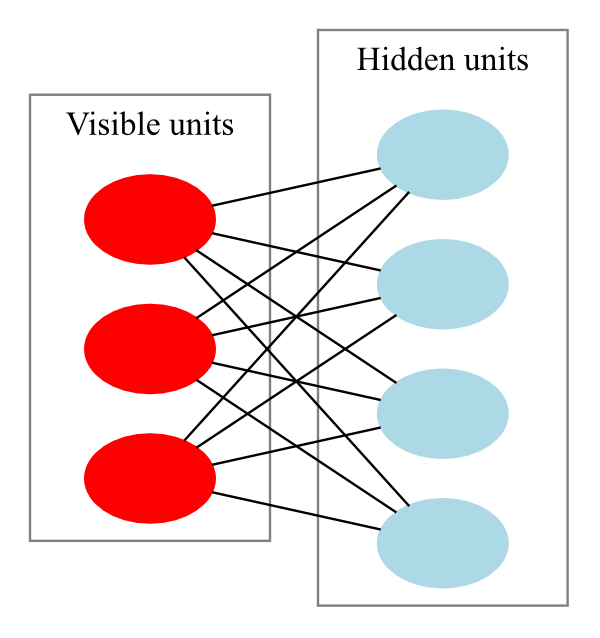
\includegraphics[width=0.45\textwidth]{restricted_boltzmann}
\caption{A Restricted Boltzmann machine.}
\end{figure}

This gives us an RBM, which is a \emph{bipartite} graph with the visible and hidden units forming distinct layers. Calculating the conditional distribution \(P(h_i | x)\) is readily tractable and now factorizes to: 
\[P(h | x) = \prod_i P(h_i | x)\]
\[P(h_i = 1 | x) = sigmoid \left( \sum_j W_{ji} x_j + d_i \right)\]

Very successful deep learning algorithms stack multiple RBMs together, where the hiddens \(h\) from the visible input data \(x\) become the new input data for another RBM for an arbitrary number of layers. 

\begin{figure}[h!]
  \centering
    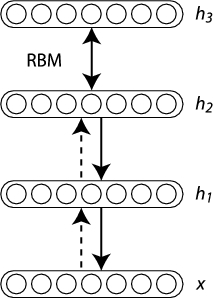
\includegraphics[width=0.3\textwidth]{stacked_rbm}
\caption{Stacked RBM.}
\end{figure}

There are a few drawbacks to the probabilistic approach to deep architectures:
\begin{enumerate}
\item The posterior distribution \(P(h_i | x)\) becomes incredibly complicated if the model has more than a few interconnected layers. We are forced to resort to sampling or approximate inference techniques to solve the distribution, which has computational and approximation error prices.
\item Calculating this distribution over latent variables still does not give a usable feature vector to train a final classifier to make this algorithm useful for AI tasks. For example, we calculate all of these hidden distributions that explain the variations over the handwriting digit recognition problem, but they do not give a final classification of a number. Actual feature values are normally derived from the distribution, taking the latent variable's expected value, which are then used as the input to a normal machine learning classifier, such as logistic regression.
\end{enumerate}

\subsection{Direct encoding models: auto-encoder}
To get around the problem of deriving useful feature values, an auto-encoder is a non-probabilistic alternative approach to deep learning where the hidden units produce usable numeric feature values. An auto-encoder directly maps an input \(x\) to a hidden layer \(h\) through a parameterized closed-form equation called an encoder. Typically, this encoder function is a nonlinear transformation of the input to \(h\) in the form:
\[f_\Theta (x) = s_f (b + Wx)\]

This resulting transformation is the feature-vector or representation computed from input \(x\).
Conversely, a decoder function is used to then map from this feature space \(h\) back to the input space, which results in a reconstruction \(x'\). This decoder is also a parameterized closed-form equation that is a nonlinear undoing the encoding function:
\[g_\Theta (h) = s_g (d + W' h)\]

In both cases, the nonlinear function s is normally an element-wise sigmoid, hyperbolic tangent nonlinearity, or rectifier linear unit.

Thus, the goal of an auto-encoder is to minimize a loss function over the reconstruction error given the training data. Model parameters \(\Theta\) are \(\left\{W,b,W',d\right\}\), with the weight matrix \(W\) most often having tied weights such that \(W' = W^T\) .

Stacking auto-encoders in layers is the same process as with RBMs.
\begin{figure}[h!]
  \centering
    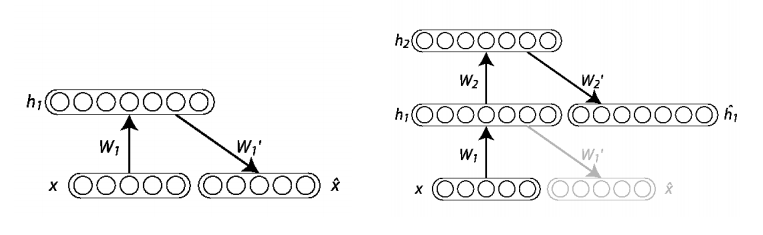
\includegraphics[width=0.8\textwidth]{stacked_autoencoder}
\caption{Stacked auto-encoder.}
\end{figure}

One disadvantage of auto-encoders is that they can easily memorize the training data (i.e. find the model parameters that map every input seen to a perfect reconstruction with zero error) given enough hidden units \(h\). To combat this problem, regularization is necessary, which gives rise to variants such as sparse auto-encoders, contractive auto-encoders, or denoising auto-encoders.

A practical advantage of auto-encoder variants is that they define a simple, tractable optimization objective that can be used to monitor progress.

\section{Denoising Auto-encoders}
Denoising auto-encoders \cite{bengio13a, vincent08} are a class of direct encoding models that use synthetic noise over the inputs through a corruption process during training to prevent overfitting and simply learning the identity function. Given a known corruption process \(C(\widetilde{X}|X)\) to corrupt an observed variable \(X\), the denoising auto-encoder learns the reverse conditional \(P(X|\widetilde{X})\). Combining this estimator with the known corruption process \(C\), it can recover a consistent estimator of \(P(X)\) through a Markov chain that alternates sampling from \(C(\widetilde{X}|X)\) and \(P(X|\widetilde{X})\). The basic algorithm is as follows:

\begin{algorithm}[h!]
	\KwIn{training set \(D\) of examples \(X\), a corruption process \(C(\widetilde{X}|X)\), and a conditional distribution \(P_\Theta(X|\widetilde{X})\) to train.}
	\While{training not converged}{
		sample training example \(X \sim D\)\;
		sample corrupted input \(\widetilde{X} \sim C(\widetilde{X}|X)\)\;
		use (\(X\),\(\widetilde{X}\)) as an additional training example towards minimizing the expected value of \(-\log P_\Theta (X|\widetilde{X})\), e.g., by a gradient step with respect to \(\Theta\) in the encoding/decoding function\;
	}
	\caption{ Generalized Denoising Auto-encoder Training Algorithm }
\end{algorithm}

